\section{Verbesserung der Augen}
\label{verbesserung_ElSe}
Zusätzlich zu den 64 Landmarks, die ein Gesicht beschreiben, kann von OpenFace weitere 28 Landmarks für ein Auge bestimmt werden, aus denen dann die Blickrichtung ermittelt wird.\\
Um die Position der Landmarks zu verbessern, kann auf dem Bildausschnitt der Augen der ElSe-Algotithmus eingesetzt werden. Dieser Algorithmus arbeitet auf einem Farbbild um so die Umrisse der Pupille zu berechnen.\\
Da unter den 28 Landmarks die Umrisse von Pupille und Iris beschreiben wird, müssen diese aus dem Ergebnis von ElSe abgeleitet werden. Dabei hat sich eine Veränderung des Radius mit ?? für Pupille und ?? für die Iris bewährt.\\
Allerdings muss das Auge für die Berechnung aus entsprechend vielen Pixeln bestehen, wodurch es im Originalbild mindestens mit 10 Pixeln dargestellt wird, um sinnvolle Ergebnisse zu erhalten. Da diese Berechnung unabhängig der Landmarks ausgeführt wird, empfiehlt sich das Ergebnis zu überprüfen, damit die bestimmte Ellipse auch innerhalb der Augenhöhle liegt.\\
Dabei wird jedes Auge unabhängig vom anderen betrachtet, wodurch sich verschiedene Blickrichtung ergeben. Ab einer Distanz von mehr als ??cm kann die Blickrichtung beider Augen als parallel angesehen und kann entsprechend behandelt werden. Eine Verbesserung ergibt sich, wenn beide Augen anhängig von einander bestimmt werden, damit sich der Fehler minimiert.
\subsection{Auswirkung der verschiedenen Verfahren - To Do}
Grafiken neu machen\\\\
Um die einzelnen Verfahren besser Vergleichen zu können wurden künstliche Augen aus dem Datensatz \cite{database_Eye} verwendet, da die Exakte Position der Landmarks bekannt sind.
Da auch in der späteren Anwendung der Augenbereich genauer bestimmt ist, bevor ElSe zum Einsatz kommt wurde, nur der Bildbereich in dem alle Landmarks der Augenlider liegen, somit sind die Bilder etwa 64 auf 29 Pixel groß. Um die Qualität der Berechnung bei verschiedenen Größen zu simulieren, wurde das Bild um den angegebenen Faktor linear verkleinert.\\
Ein gutes Verfahren muss stabil gegenüber der Skalierung sein damit es auch auf kleinen Bereichen zuverlässig arbeitet. Da für die spätere Anwendung vor allem das Zentrum der Pupille von Interesse ist, wird der Abstand zum Zentrum als Qualitätsmaß verwendet.\\
\begin{figure}
	\centering
	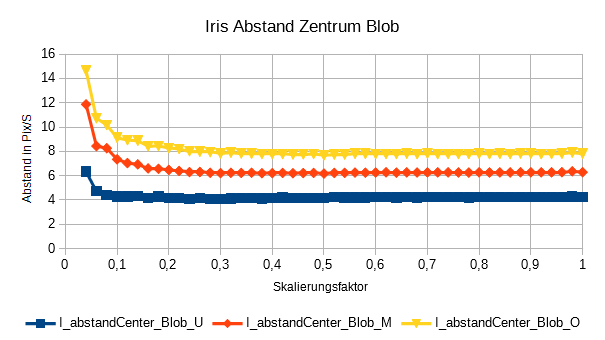
\includegraphics[width=0.49\linewidth]{Eye_Img/ElSe_22Gray_Iris_Zentrum}
	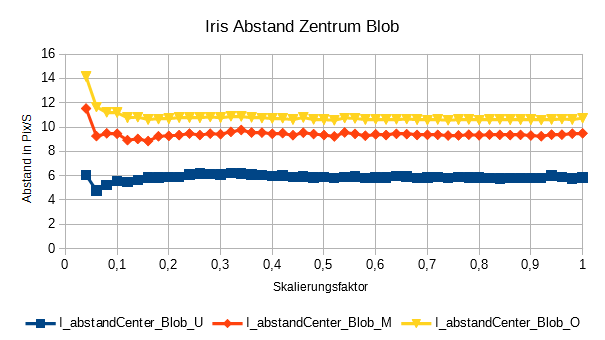
\includegraphics[width=0.49\linewidth]{Eye_Img/ElSe_22N1Gray_Iris_Zentrum}
	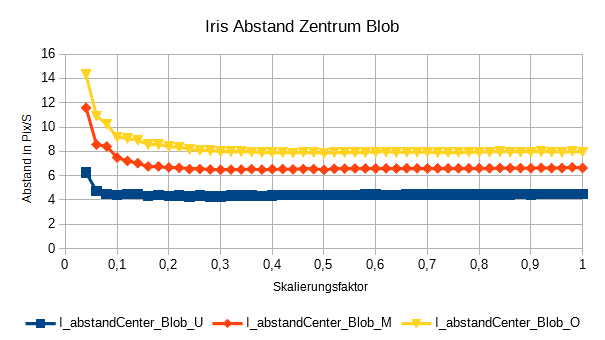
\includegraphics[width=0.49\linewidth]{Eye_Img/ElSe_New_Iris_Zentrum}
	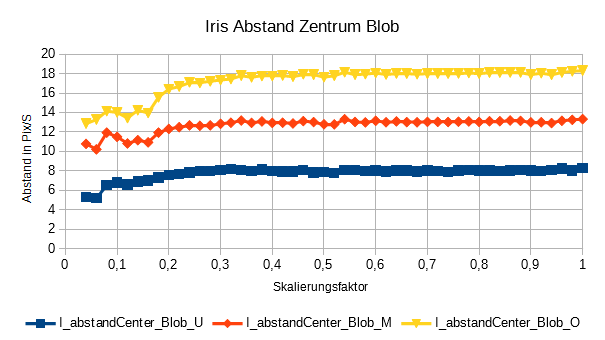
\includegraphics[width=0.49\linewidth]{Eye_Img/ElSe_MaxGray_Iris_Zentrum}
	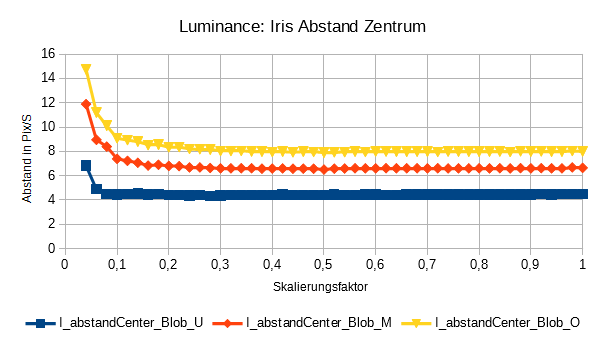
\includegraphics[width=0.49\linewidth]{Eye_Img/ElSe_Norm_Iris_Zentrum}
	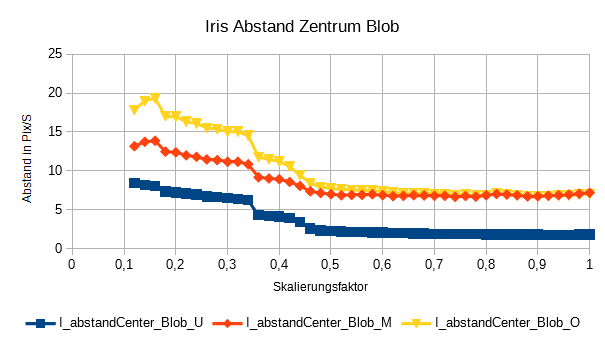
\includegraphics[width=0.49\linewidth]{Eye_Img/OpenFace_Iris_Abstand}
	\caption{Abstand des Zentrums der Landmark-Pupille und der Berechneten Ellipse in [Pixel/Skalierung] Oben-Links: Gleam, Oben-Rechts: Gleam mit 1, Mitte-Links: Gleam New, Mitte-Rechts: Max-Wert, Unten-Links: Luminance, Unten-Rechts: OpenFace}
	\label{ElSe_Gray_Zentrum}
\end{figure}
\begin{figure}
	\centering
	\centering
	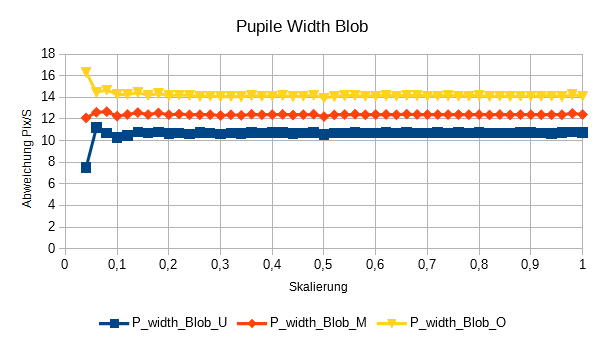
\includegraphics[width=0.49\linewidth]{Eye_Img/ElSe_22Gray_Pupile_Width}
	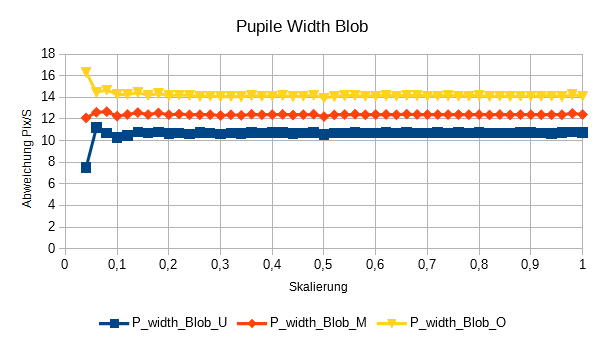
\includegraphics[width=0.49\linewidth]{Eye_Img/ElSe_22N1Gray_Pupile_Width}
	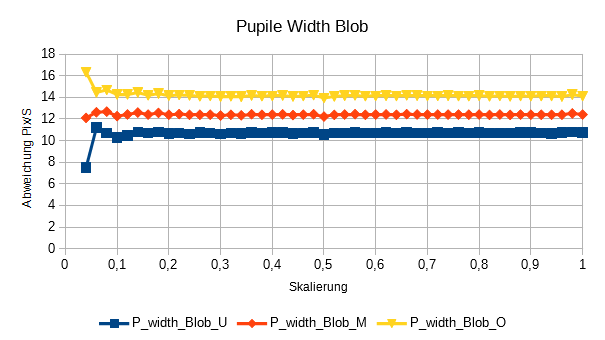
\includegraphics[width=0.49\linewidth]{Eye_Img/ElSe_New_Pupile_Width}
	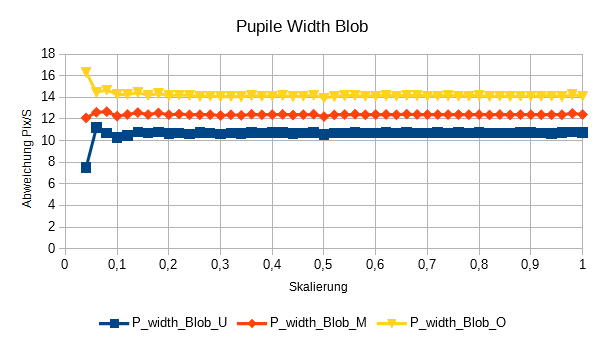
\includegraphics[width=0.49\linewidth]{Eye_Img/ElSe_MaxGray_Pupil_Width}
	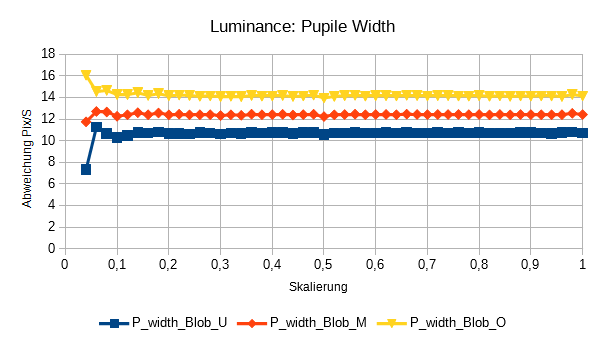
\includegraphics[width=0.49\linewidth]{Eye_Img/ElSe_Norm_Pupil_Width}
	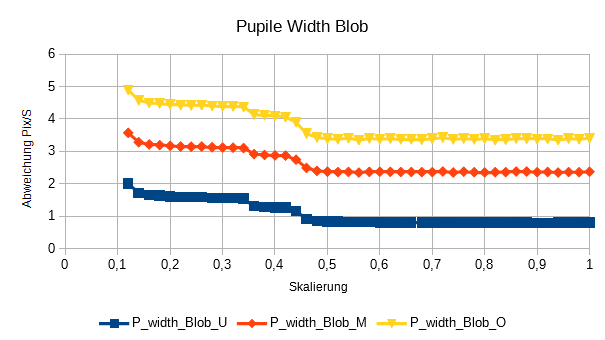
\includegraphics[width=0.49\linewidth]{Eye_Img/OpenFace_Pupile_Width}
	\caption{Unterschied Zwischen den Radien der Landmark-Pupille und der Berechneten Ellipse in [Pixel/Skalierung] Oben-Links: Gleam, Oben-Rechts: Gleam mit 1, Mitte-Links: Gleam New, Mitte-Rechts: Max-Wert, Unten-Links: Luminance, Unten-Rechts: OpenFace}
	\label{ElSe_Gray_Width}
\end{figure}
\begin{figure}
	\centering
	\centering
	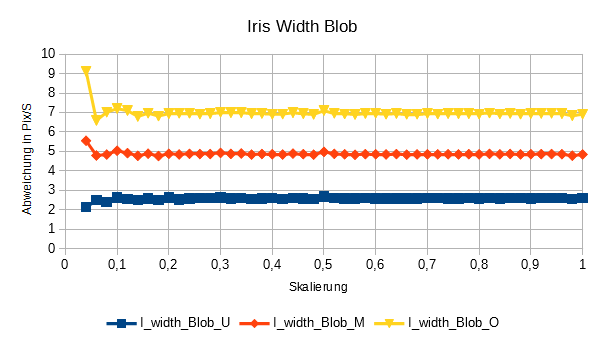
\includegraphics[width=0.49\linewidth]{Eye_Img/ElSe_22Gray_Iris_Width}
	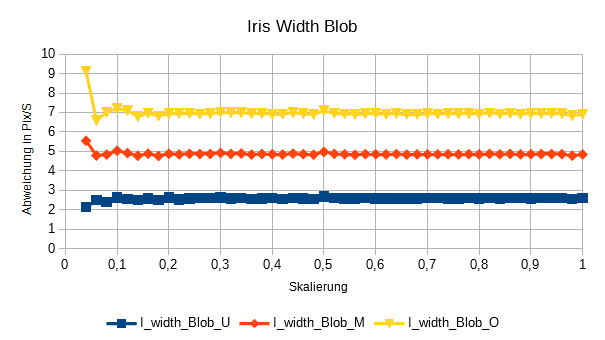
\includegraphics[width=0.49\linewidth]{Eye_Img/ElSe_22N1Gray_Iris_Width}
	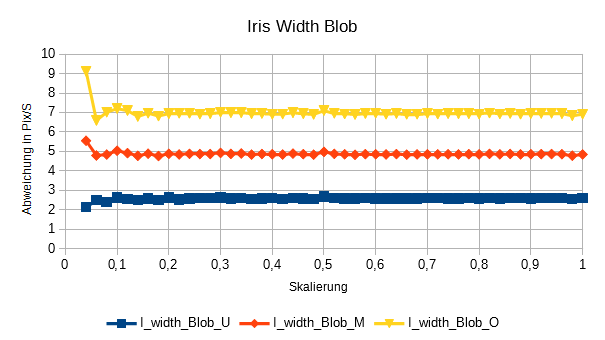
\includegraphics[width=0.49\linewidth]{Eye_Img/ElSe_New_Iris_Width}
	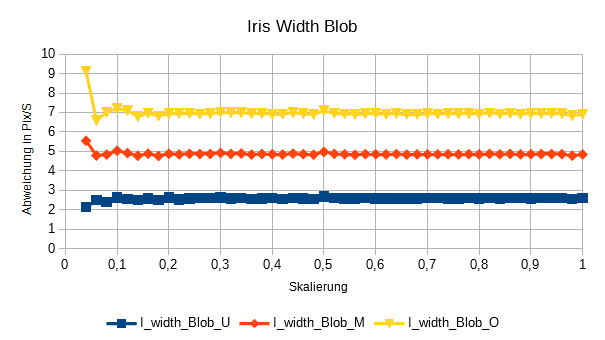
\includegraphics[width=0.49\linewidth]{Eye_Img/ElSe_MaxGray_Iris_Width}
	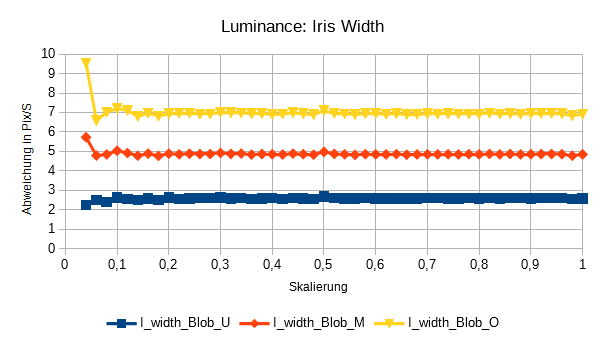
\includegraphics[width=0.49\linewidth]{Eye_Img/ElSe_Norm_Iris_Width}
	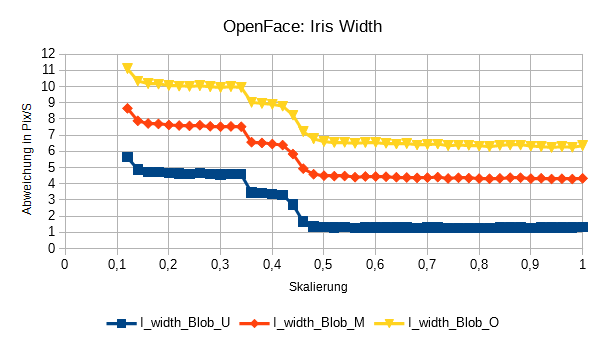
\includegraphics[width=0.49\linewidth]{Eye_Img/OpenFace_Iris_Width}
	\caption{Unterschied Zwischen den Radien der Landmark-Iris und der Berechneten Ellipse in [Pixel/Skalierung] Oben-Links: Gleam, Oben-Rechts: Gleam mit 1, Mitte-Links: Gleam New, Mitte-Rechts: Max-Wert, Unten-Links: Luminance, Unten-Rechts: OpenFace}
	\label{ElSe_Gray_Iris}
\end{figure}
Es Zeigt sich, dass das Verfahren um den Farbwert in einen Grauwert zu überführen durchaus Auswirkungen vor allem auf die Positionsbestimmung hat. Vor allem Verfahren, die das Graubild aufhellen, liefern schlechtere Ergebnisse.\\
Außerdem arbeitet ElSe stabil bei den Skalierungen, womit es vor allem auch bei kleinen Bildern zuverlässig Ergebnisse liefern kann.\\
Da die Abweichung von ElSe konstant bei etwa 6.5 liegt, ist es bei kleineren Bildern OpenFace überlegen. So ist im Test der Durchschnitt bei alles Skalierungen ElSe den Ergebnisse von OpenFace überlegen, durch die Verteilung ist allerdings eine Kombination beider Verfahren sinnvoll, so kann das Ergebnis von OpenFace bei Bilder in denen die Iris größer als 16 Pixel ist als Lösung verwendet werden. Im Bereich zwischen 12 und 16 Pixel können beide Ergebnisse Kombiniert werden, sollte die Iris im Originalbild noch kleiner sein, so ist auf ElSe mehr verlass, da es noch bis zu einer Irisgröße von 3 Pixel noch stabil funktioniert.
\subsection{ElSe - Auswirkung des Radius - To Do}
Ein weiter wichtiger Parameter des ElSe-Verfahrens ist der Radius des Filters. Wiederrum wurde der Augen-Datensatz \cite{database_Eye} verwendet und das Auge ausgeschnitten um diesen Bereich auf 384 Pixel als Eingabebild für ElSe zu vergrößern. Die Umwandlung von Farb- nach Grau-Wert wurde mit dem Luminance-Verfahren eingesetzt.\\
Im Datensatz besitzen die abgebildeten Augen eine Durchschnittlich Pupille von 15 Pixel und eine Iris von 34 Pixel.
\begin{figure}
	\centering
	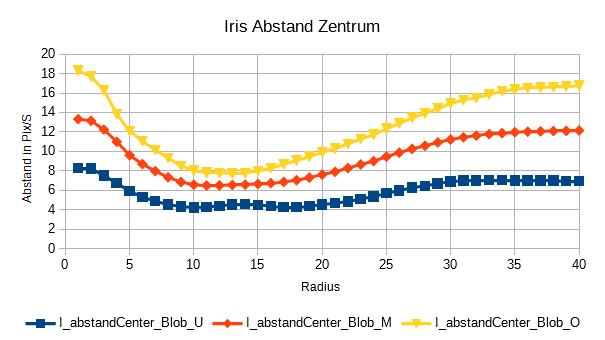
\includegraphics[width=0.49\linewidth]{Eye_Img/Radius_Iris_Zentrum}
	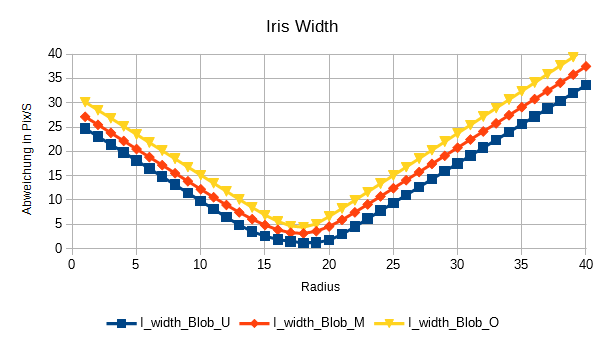
\includegraphics[width=0.49\linewidth]{Eye_Img/Radius_Iris_Width}
	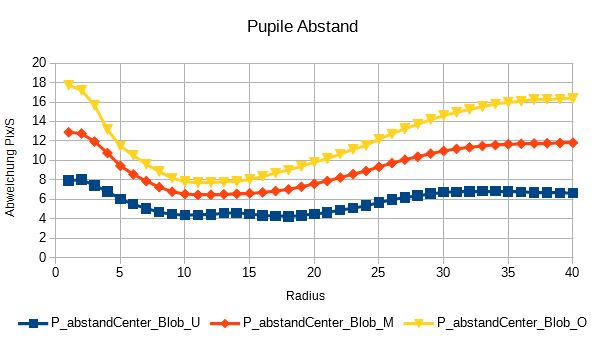
\includegraphics[width=0.49\linewidth]{Eye_Img/Radius_Pupile_Zentrum}
	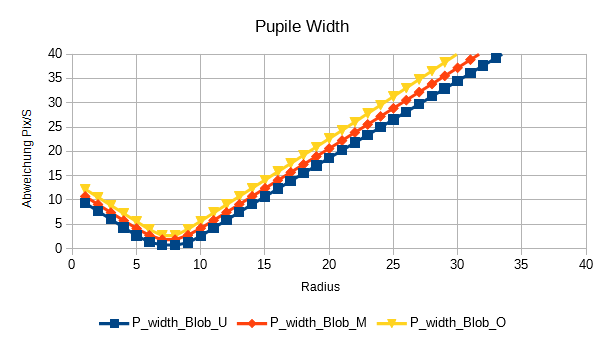
\includegraphics[width=0.49\linewidth]{Eye_Img/Radius_Pupile_Width}
	\caption{Auswirkung bei der Veränderung des Radius des ElSe-Algorithmus}
	\label{ElSE_Radius}
\end{figure}
Es ist zu erkennen, dass die Wahl des Radius signifikant ist für die Qualität der Berechnung. Da für die spätere Anwendung vor allem das Zentrum der Pupille von Interesse ist, siehe \autoref{OpenFace_Blickrichtung}, muss ElSe in diesem Aspekt stabil gegenüber der Skalierung sein.\\
Im Versuch hat sich ein Radius von etwa einem Zehntel des zu erwartetem Durchmesser der Iris bzw. Pupille als sinnvoll erwiesen, siehe \autoref{ElSE_Radius}. Um ein möglichst robustes Verfahren zu erhalten.
Dabei ist zu erwähnen das eine Differenzierung zwischen Iris und Pupille meist nicht möglich ist, da der Farbunterschied recht gering ist und deutlich weniger als der Grauwert vom Rest des Auges.\\
\subsection{OpenFace - Auge To Do}
Als Referenz wir das Ergebnis von OpenFace für die zusätzlich bestimmten Landmarks der Augen verwendet. Dies wurde auch auf dem Augendatensatz \cite{database_Eye} angewendet um vergleichbare Ergebnisse zu erhalten.
\begin{figure}
	\centering
	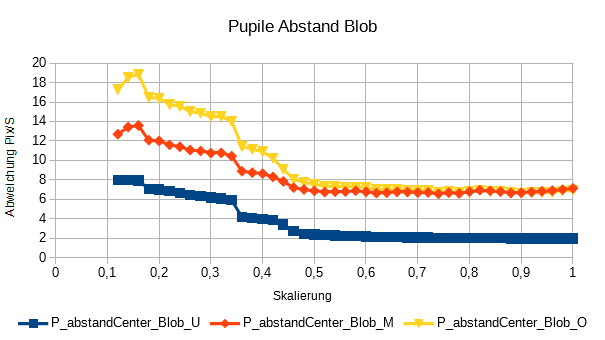
\includegraphics[width=0.45\linewidth]{Eye_Img/OpenFace_Pupile_Abstand}
	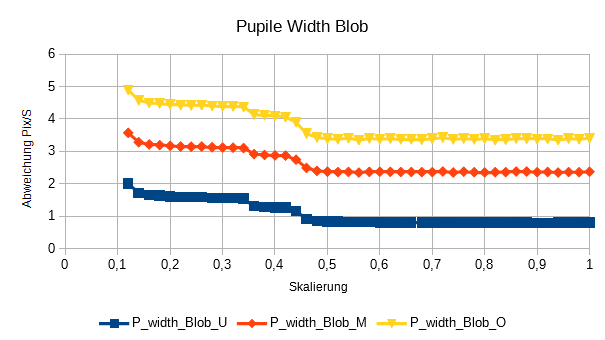
\includegraphics[width=0.45\linewidth]{Eye_Img/OpenFace_Pupile_Width}
	\caption{Auswirkung von Skalierung auf die Qualität der Augendetektion von ObenFace}
	\label{OpenFace_Eye}
\end{figure}
Es ist zu erkennen dass dieses Verfahren im schnitt oft schlechtere Ergebnisse liefert als das Ergebnis von ElSe, allerdings ohne das begehen von großen Fehlern und auch öfters genauere Ergebnisse.\\
Somit ist eine Kombination beider Verfahren von Vorteil, vor allem bei kleinen Bildern kann eine erneute Bestimmung der Pupille von Vorteil.
\begin{itemize}
	\item Grafik neu
	\item Vergleich zu ElSe
\end{itemize}

